\documentclass{article}
\usepackage[utf8]{inputenc}
\usepackage{amsmath,amsfonts,amssymb,amsthm,mathtools}
\usepackage{parskip}
\usepackage{color}
\usepackage{booktabs}
\usepackage{hyperref}
\usepackage{tikz}
\usetikzlibrary{shapes,arrows,positioning,calc,fit,backgrounds,matrix,decorations.pathmorphing}
\definecolor{attentiontarget}{RGB}{180,180,180}
\usepackage[framemethod=tikz]{mdframed}
\usepackage{float}
\usepackage{placeins}
\usepackage{subcaption}
\usepackage{graphicx}

\definecolor{blue}{RGB}{38,139,210}
\definecolor{cyan}{RGB}{42,161,152}
\definecolor{violet}{RGB}{108,113,196}
\definecolor{red}{RGB}{220,50,47}
\definecolor{base01}{RGB}{88,110,117}
\definecolor{base02}{RGB}{7,54,66}
\definecolor{base03}{RGB}{0,43,54}

\usetikzlibrary{calc,shapes,positioning}

\newtheorem{exercise}{Exercise}
\newtheorem{answer}{Answer}

\newcommand{\dd}[2][]{\frac{\partial #1}{\partial #2}}
\newcommand{\dt}[2][]{\frac{d #1}{d #2}}
\newcommand{\dL}{\dt[{\L}]}
\newcommand{\dLi}{\dt[{\Li}]}
\newcommand{\dLmb}{\dt[{\Lmb}]}
\newcommand{\dLfb}{\dt[{\Lfb}]}
\newcommand{\yh}{\hat{y}}

\newcommand{\x}{\mathbf{x}}
\newcommand{\y}{\mathbf{y}}
\newcommand{\logits}{\ell}
\newcommand{\vlogits}{\boldsymbol{\logits}}

\newcommand{\bracket}[3]{\left#1 #3 \right#2}
\newcommand{\sqb}{\bracket{[}{]}}
\newcommand{\ab}{\bracket{\langle}{\rangle}}
\renewcommand{\b}{\bracket{(}{)}}
\newcommand{\abs}{\bracket{\lvert}{\rvert}}

\newcommand{\W}{\mathbf{W}}
\newcommand{\Wkey}{\mathbf{W}_\text{k}}
\newcommand{\Wquery}{\mathbf{W}_\text{q}}
\newcommand{\A}{\mathbf{A}}
\newcommand{\B}{\mathbf{B}}
\newcommand{\X}{\mathbf{X}}
\newcommand{\Y}{\mathbf{Y}}
\renewcommand{\H}{\mathbf{H}}
\renewcommand{\a}{\mathbf{a}}
\newcommand{\h}{\mathbf{h}}
\newcommand{\p}{\mathbf{p}}




\title{SEMT20003: Large Language Models}
\author{Laurence Aitchison}
\date{}

\begin{document}

\maketitle

One of the most impressive developments in modern AI is ``Large Language Models'' (LLMs).
This week, we're going to look at the basic building blocks that make LLMs such as ChatGPT work.

\section{How text is represented in the computer}

Text is represented in programming as a ``string''.
For instance, if you do:
\begin{verbatim}
>>> a = "Fine tuning is fun for all!"
\end{verbatim}
That's a string.
You can do various operations on strings.  For instance, we can take the first 10 characters:
\begin{verbatim}
>>> a[:10]
"Fine tunin"
\end{verbatim}
See notebooks for more details.

\section{Tokenisation}

Neural networks work with numbers, not text/strings.
So first question is: how do we convert text/strings to numbers (and back).
The answer is ``tokenization''.

In tokenization, we associate substrings (usually but not always words) such as `` is'' with an integer index.
As an example:
\begin{center}
  \includegraphics[width=0.6\textwidth]{token_small.png}
\end{center}
Each coloured substring is a token, represented by an integer.
We can therefore map from a string to a sequence of tokens and back.
There's a larger example below:
\begin{center}
  \includegraphics[width=0.9\textwidth]{token_big.png}
\end{center}
By this point, tokenization is handled by low-level libraries, so we're not going to worry about it more here.

\section{LLMs do classification to predict the next token}

One of the most common things people say about LLMs is that they ``just predict the next token''.
That's true.
In fact, LLMs really just do \textbf{classification} to predict the next token (word), given the previous tokens (words).
This notion of classification makes sense, because a token just looks like an integer class-label; so ``class 103'' means ``after these tokens (words), I expect token (word) 103 to come next''.

Remember that when we introduced the loss function for classification, we did it through a probabilistic perspective.
The probability that next token is $y$ (or equivalently that the ``class-label'' is $y$) given the previous tokens, $\x$, is,
\begin{align}
  p_y(\x) &= \frac{\exp\b{\logits_y(\x)}}{\sum_{c=1}^C \exp\b{\logits_c(\x)}}
\end{align}
Here, $\logits_c(\x)$ is the output of the neural network, which is one number for each possible token, and $C$ is the total number of tokens (usually about 50,000 in modern LLMs).

This probabilistic perspective is \textit{really} important in LLMs.
You often don't want the LLM to always return the same token given the same input (or ``prompt'').
For instance, you might want your model to generate a bunch of different stories, so that you can then pick the best one.
That obviously won't work if the LLM always produces the same story!
So usually, instead of just taking the highest probability token, we will usually \textit{randomly sample} from the distribution represented by $p_y(\x)$.
Sampling tends to give us better ``more creative'' text, while taking the most likely token tends to give ``more boring'' text.

This contrasts with classification.  In particular, when we were doing classification, we frequently didn't care about the distribution.
Instead, we just cared about the most likely class.
As such, we pretty rapidly dropped the probabilistic interpretation.

\section{Embedding}

We've converted text/a string to a list of integer tokens:
\begin{enumerate}
  \item Start off with some text: \verb|"This is a string"|.
  \item Tokenize (i.e. convert to a list of tokens/integers): \verb|[1023, 932, 12, 6433]|.
\end{enumerate}
At least this is numbers, so its closer to something that we can put in a neural network.
While we could (technically) put integers directly into a neural network, it won't work well.
That's because neural networks fundamentally process vectors.
So what we really want is one vector for each token/word.
That makes alot of sense if we remember that in images, we had one vector for each pixel.

That means we need to convert tokens to vectors.
We basically use a giant look-up table to convert tokens to vectors.
This look-up table is a giant matrix of shape $C \times H$, where $C$ is the total number of tokens and $H$ is the ``embedding dimension'', or the length of the vector associated with each token.
 
Once we look up a sequence of tokens in the giant look-up table, we end up with a $S \times H$ matrix, where $S$ is the sequence length.

Thus the process of converting text into vectors that are suitable for putting into a neural network is:
\begin{enumerate}
  \item Start off with some text: \verb|"This is a string"|.
  \item Tokenize (i.e. convert to a list of tokens/integers): \verb|[1023, 932, 12, 6433]|.
  \item Embed the tokens to get a $S\times H$ matrix (here, $S = 4$, and remember that $H$ is the embedding dimension).
\end{enumerate}

\section{Problems with convolutional networks for text}

You can think of the $S \times H$ embedding as being like a feature-map in a convolutional network.
In a convolutional network, we have one vector associated with each pixel, while here we have one vector associated with each token/word.
Now comes the question of how to use neural-networks to transform these features.
One option is convolutional networks.
Specifically, 1D convolutions, where we treat $S$ as the only ``spatial'' dimension.

The problem with sentences is that dependencies work in strange ways.
Consider the following sentence:
\begin{verbatim}
  Alice and Bob introduced themselves.  She said "my name is
\end{verbatim}
Its fairly obvious that the most likely next word is be ``Alice''.
That's because that ``She'' is likely (but not certain) to refer to Alice.
However, this dependency is really hard to embed in a convolutional architecture:
\begin{itemize}
  \item The token ``Alice'' could be an arbitrary number of tokens back.
  \item Whether we care most about the ``Alice'' or ``Bob'' token is super complicated. Its depends on the token ``She'', along with the model's judgement about the probability of Alice and Bob being boy's / girl's names.
\end{itemize}
Convolutions certainly can't understand these super-flexible dependencies, as they just consider a fixed region.
Indeed, people tried convolutional networks, and they don't work well.

%\section{Attention: high level}
%
%In the above example, we know that ``She'' probably refers to ``Alice'', so we somehow want the feature-vector for ``She'' to look like the feature-vector for ``Alice''.
%Attention layers let us do that.
%Attention layers:
%\begin{itemize}
%  \item Map from an $S \times H$ input matrix, $\X$,
%  \item to a $S \times H$ output matrix, $\Y$,
%  \item Use an $S \times S$ matrix of attention weights, $\A(\X)$, which is a function of the inputs, $\X$.
%\end{itemize}
%Note that usually, we use $\X$ and $\Y$ as in the inputs and outputs of a whole network; while here we're going to use them as the inputs and outputs of a single layer.
%We can write the expression for attention in three equivalent forms:
%Fully in index notation:
%\begin{align}
%  \label{eq:att_idx}
%  Y_{i \lambda} &= \sum_{j=1}^S A_{ij}(\X) X_{j \lambda}
%\end{align}
%Here, $i$ and $j$ range from $1$ to $S$ and index tokens.  In contrast, $\lambda$ ranges from $1$ to $H$ and indexes the feature/channel.
%With vectors, (taking $\y_i = Y_{i, :}$ and $\x_j = X_{j, :}$),
%\begin{align}
%  \label{eq:att_vec}
%  \y_i &= \sum_{j=1}^S A_{ij}(\X) \x_{j}
%\end{align}
%where $\x_{j}$ is the input feature vector associated with token $j$, and $\y_i$ is the output feature vector associated with token $i$.
%Finally, we can write the expression in matrix form,
%\begin{align}
%  \label{eq:att_mat}
%  \Y &= \A(\X) \X.
%\end{align}
%To get intuition for what this expression is doing, its easiest to look at the expression with vectors (Eq.~\ref{eq:att_vec}).
%The attention weights are almost always positive, 
%\begin{align}
%  0 &\leq A_{ij}(\X)
%\end{align}
%In that case, the sum in Eq.~\eqref{eq:att_vec} is saying that the $i$th output, $\y_i$, is a mixture of the input features describing the other tokens, $\x_j$. 
%That mixture has weights, $A_{i, j}(\X)$, describing how much of each feature to mix into to output $\y_i$.
%Critically, the weights for that mixture are flexible, and can choose to emphasise particular tokens and ignore others.
%As an example:
%
%\begin{center}
%\begin{minipage}{0.6\textwidth}
%  $\quad \quad \quad \quad \x_j \quad\quad\quad\quad \quad \quad \quad \quad \quad \quad \quad \y_i$
%
%  \includegraphics[width=\textwidth]{self_attention_crop}
%\end{minipage}
%\end{center}

%\section{Attention: how to choose the attention weights}
%
%The previous section on attention describes the key idea behind attention: its always about mixing together tokens in a flexible way.
%However, in the previous section, we left open a critical question: how exactly do we choose the attention weights, $\A(\X)$?
%It turns out is an active area of research, and there are lots of different proposals.
%However, in these notes, we'll focus on the single most common approach (which is used in all the largest-scale LLMs).
%
%The first thing we need is to work out how we get a $S \times S$ matrix from $\X$.  The answer is:
%\begin{align}
%  \underbrace{\B(\X)}_{S \times S} &= \underbrace{\X}_{S \times H} \underbrace{\W}_{H \times H} \underbrace{\X^T}_{H \times S}
%\end{align}
%here, $\W$ is learned weight parameters.
%Now, we're almost there: $\B$ is $S \times S$; which is the same size that we need for $\A(\X)$.
%The only issue is that the elements of $\B$ could be positive or negative, whereas in the previous section we said that we wanted the attention weights to always be positive.
%We therefore apply some kind of nonlinearity.
%The nonlinearity people usually use is softmax,
%\begin{align}
%  \A(\X) &= \text{softmax}\b{\B(\X), \text{axis}{=}-1}\\
%  \A(\X) &= \text{softmax}\b{\X \W \X^T, \text{axis}{=}-1}.
%\end{align}
%Weirdly, this is the same function (softmax) that we used to get the class probabilities for classification.
%Remembering the definition of the softmax, this gives:
%\begin{align}
%  A_{ij} &= \frac{\exp\b{B_{ij}}}{\sum_{j'=1}^S \exp\b{B_{ij'}}}
%\end{align}
%(the $\text{axis}{=}-1$ tells us to do the sum in the denominator over the second index, $j$, rather than the first index, $i$).
%The use of the softmax means that the attention weights, $\A(\X)$ have two properties:
%\begin{itemize}
%  \item They're positive.
%  \item They sum to $1$ ($1=\sum_j A_{ij}(\X)$).
%\end{itemize}
%These properties make the attention look a bit like probabilities.
%But they aren't probabilities.
%That's because for it to be probabilities, we need a discrete random variable which takes values from $1$ to $S$ with probabilities given by $A_{i:}(\X)$, and we don't have such a random variable.
%Instead, $A_{i:}(\X)$ just specifies the mixture weights. 
%Indeed, as mentioned in the previous section, the attention weights don't have to normalize to $1$: people can and often do use attention weights that don't normalize, and they don't look like probabilities at all.

\section{Attention as lookup}

In the earlier example, we know that ``She'' probably refers to ``Alice'', so we somehow want the feature-vector for ``She'' to incorporate information from the feature-vector for ``Alice''. When attention gets to ``She'', it ``looks up'' information from ``Alice''!
Note that ``attention'' is the term people in deep learning use.
But I actually think that the operation is best understood as ``lookup'', so I'll be using both terms here.

\subsection{Simple examples of look-up/attention operations}
A look-up operation has two things: the query and the key/value pairs.

To understand the key/value pairs, lets consider a couple of examples.

First, consider a dictionary (i.e.\ the big book that gives the definitions of all the words).
This entire book is just a massive list of key/value pairs, where:
\begin{itemize}
  \item The keys are the words.
  \item The values are the corresponding definitions.
\end{itemize}
As another example, consider a phone-book (a book you sometimes see in old films that you'd use to lookup people's phone numbers).  This is also a massive list of key/value pairs.  But this time:
\begin{itemize}
  \item The keys are people's names.
  \item The values are their phone numbers.
\end{itemize}
So a phone-book looks like:
\begin{center}
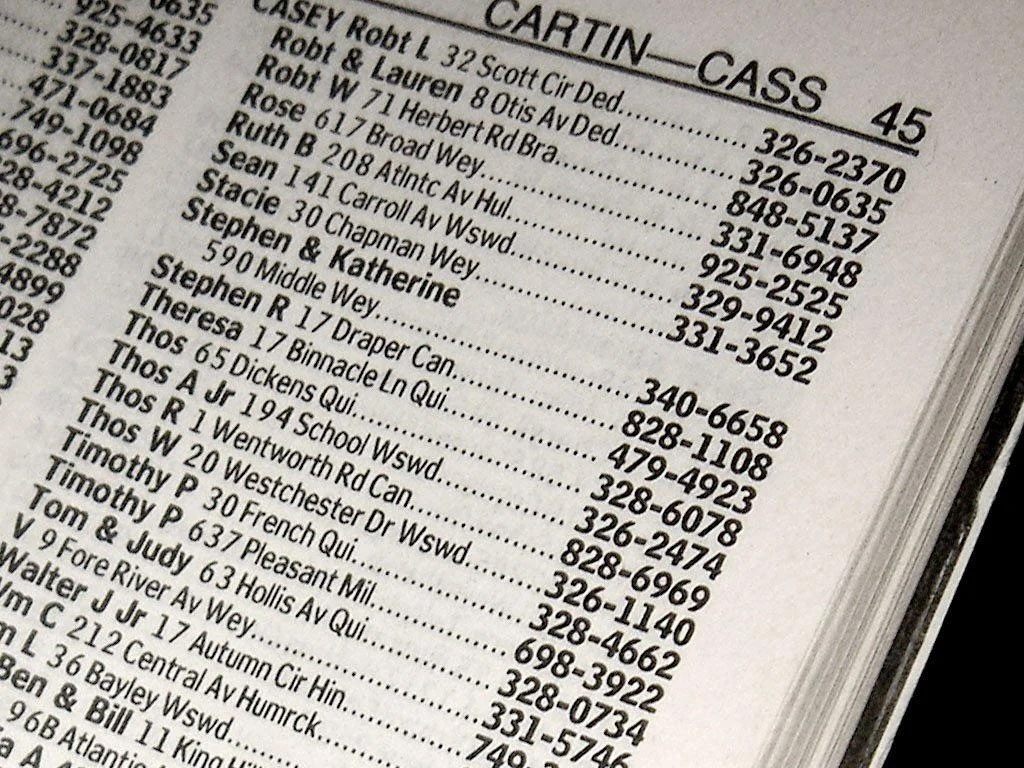
\includegraphics[width=0.6\textwidth]{phone_book}
\end{center}
In both cases, the query is ``what we're looking for''.  So:
\begin{itemize}
  \item For a dictionary, the query is the word who's definition we're looking up.
  \item For the phone book, the query is the name of the person who's phone number we're looking up.
\end{itemize}

\subsection{Look-up/attention as a Python dictionary}

This query and key/value pair terminology was initially inspired by something like Python's dictionary datastructure.
You construct a dictionary using a list of keys and values:
\begin{verbatim}
dictionary = {} # initialize an empty dictionary.
for key, value in zip(key, value):
    dictionary[key] = value # insert a key-value pair into the dictionary.
\end{verbatim}
Then you can look up a particular query:
\begin{verbatim}
result = dictionary[query]
\end{verbatim}
If query is equal to one of the keys, then you'll get the value corresponding to that key.
In Python, if the query isn't equal to any of the keys, you get an error.

\subsection{Look-up/attention as a mathematical operation}

That's Python code.  We need to make things more mathematical.
We start by saying that the query, $\mathbf{q}$, is a vector, and each key and value is also a vector.
We have a collection of $S$ key/value pairs (e.g. in the phone-book example, $S$ is the number of people in the phone-book), so we collect the keys and values into matrices with $S$ rows 
\begin{itemize}
  \item $\mathbf{q}$ (Query): $1 \times D$
  \item $\mathbf{K}$ (Keys): $S \times D$
  \item $\mathbf{V}$ (Values): $S \times D_v$
\end{itemize}
Notice that queries and keys have the same dimension, $D$, because we're going to be interested in whether the query is the same as or similar to a particular key, which only makes sense if they have the same dimension.
But the values can have arbitrary dimension.
Now, we can write an ``identical lookup'' as,
\begin{align}
  \text{identical lookup}(\mathbf{q}, \mathbf{K}, \mathbf{V}) &= \begin{cases}
    \mathbf{V}_{j, :} & \text{if } \mathbf{K}_{j, :} = \mathbf{q}\\
    \text{undefined} & \text{otherwise}
  \end{cases}
\end{align}
i.e.\ this ``identical lookup'' operation returns the vector, $\mathbf{V}_{j, :}$ if the query is exactly equal to the corresponding key, $\mathbf{K}_{j, :}$, and is undefined if the query isn't equal to any of the keys.

Now, we can't use this ``identical lookup'' operation in a neural network, because the query is basically never going to be \textit{exactly} equal to one of the keys.
Thus, a useful alternative would be to return the value corresponding to the key that is \textit{closest} to the query,
\begin{align}
  \text{nearest lookup}(\mathbf{q}, \mathbf{K}, \mathbf{V}) &= \sum_j a^\text{nearest}_j(\mathbf{q}, \mathbf{K})\mathbf{V}_{j, :}.
\end{align}
To implement this operation, we introduced an ``attention vector'', $a^\text{nearest}_j(\mathbf{q}, \mathbf{K})$.
This vector has $S$ entries, one for each key/value pair.
It is $1$ for the key/value pair with the key closest to $\mathbf{q}$, and is zero otherwise,
\begin{align}
  a^\text{nearest}_j(\mathbf{q}, \mathbf{K}) &= \begin{cases}
    1 & \text{if $K_{j, :}$ is the closest key to $\mathbf{q}$}\\
    0 & \text{otherwise}
  \end{cases}
\end{align}
This is better, in that it is defined everywhere.

However, nearest lookup still isn't helpful for neural networks, because it isn't differentiable.
Specifically, as we move around the query, $\mathbf{q}$, it will shift from being closest to one key vector, $\mathbf{K}_{j, :}$ to being closest to another key vector, $\mathbf{K}_{j', :}$.
At that point, the output will jump from $\mathbf{V}_{j, :}$ to $\mathbf{V}_{j', :}$.
And that jump isn't differentiable.
So can we do something else?
We can do a ``soft lookup'' operation, which is exactly the same as above for the nearest lookup, but $a_j$ can be any value between $0$ and $1$, so we end up ``mixing together'' different values,
\begin{align}
  \label{eq:soft_lookup}
  \text{soft lookup}(\mathbf{q}, \mathbf{K}, \mathbf{V}) &= \sum_j a^\text{soft}_j(\mathbf{q}, \mathbf{K})\mathbf{V}_{j, :}
\end{align}
This soft attention usually (but not always) satisfies:
\begin{subequations}
\label{eq:att_as_prob}
\begin{align}
  1 = \sum_j a^\text{soft}_j(\mathbf{q}, \mathbf{K})\\
  0 < a^\text{soft}_i(\mathbf{q}, \mathbf{K}).
\end{align}
\end{subequations}
So $a^\text{soft}_j(\mathbf{q}, \mathbf{K})$ looks a bit like a probability distribution over key/value pairs
But it isn't really a probability distribution, as we don't ever sample a key/value pair from it.
Instead, Eq.~\eqref{eq:soft_lookup} uses $a^\text{soft}_j(\mathbf{q}, \mathbf{K})$ as the weights in a weighted average.
Here, the weights $a^\text{soft}_j(\mathbf{q}, \mathbf{K})$, are larger if the query is close to the key, and smaller if the query is further from the key.


How do we implement $a^\text{soft}_j(\mathbf{q}, \mathbf{K})$?
You can do lots of things.
But the most typical approach is,
\begin{align}
  a_j^\text{soft}(\mathbf{q}, \mathbf{K}) &= \frac{\exp(\mathbf{q} \cdot \mathbf{K}_{j, :})}{\sum_k \exp(\mathbf{q} \cdot \mathbf{K}_{k, :})}
\end{align}
In which case, both the properties in Eq.~\eqref{eq:att_as_prob}.

\section{Lookup/attention in LLMs}

\subsection{Self vs Cross attention}

To apply self-attention in LLMs, the key questions are:
\begin{itemize}
  \item Where do the queries come from?
  \item Where do the key/value pairs come from?
\end{itemize}
The answer to both these questions is ``tokens'':
\begin{itemize}
  \item There is one query for each token.
  \item There is one key/value pair for each token.
\end{itemize}
This is where the ``self'' in ``self-attention'' comes from: there's the same number of queries and key/value pairs, as the queries and key/value pairs are computed from the same thing: tokens.
We can also have cross attention, where the queries and key-value pairs come from different places.
For instance, the queries could be text tokens, while the key-value pairs could come from an image.

So how do we actually compute the query/key/value vector for each token in self-attention?
The answer is that we have as one vector for each token as an input.
These vectors are collected together into a matrix, $\mathbf{X}$, which is $S \times H$, where $S$ is the sequence length, and $H$ is the size of each vector.
Then, to get the queries/keys/values, we just multiply $\mathbf{X}$ by three different matrices,
\begin{align}
  \mathbf{Q} &= \mathbf{X}\mathbf{W}_q \quad \text{where } \mathbf{W}_q \text{ is } H \times D\\
  \mathbf{K} &= \mathbf{X}\mathbf{W}_k \quad \text{where } \mathbf{W}_k \text{ is } H \times D\\
  \mathbf{V} &= \mathbf{X}\mathbf{W}_v \quad \text{where } \mathbf{W}_v \text{ is } H \times D_v
\end{align}
Then we can throw one token's query, along with all key/values pairs into a standard attention/lookup operation described above.
Ultimately, each token, indexed $i$, is going to do its own lookup, so we have $S$ lookup operations in total,
\begin{align}
  \text{self-attention}_{i, :}(\mathbf{Q}, \mathbf{K}, \mathbf{V}) &= \text{soft lookup}(\mathbf{Q}_{i, :}, \mathbf{K}, \mathbf{V}) = \sum_j A_{ij}(\mathbf{Q}, \mathbf{K}) V_{j, :}
  \intertext{where we would usually, but not always, have,}
  A_{ij}(\mathbf{Q}, \mathbf{K}) &= \frac{\exp(\mathbf{Q}_{i, :} \cdot \mathbf{K}_{j, :})}{\sum_k \exp(\mathbf{Q}_{i, :} \cdot \mathbf{K}_{k, :})}
\end{align}
Here, $A_{ij}$ is the ``attention matrix''.  It tells us which tokens, $j$, each token, $i$, attends to.

\subsection{Causal vs full self-attention}

There is one final trick to self-attention.
In the diagram below, the token ``\_it'' is attending to tokens in the past, and tokens in the future.

\begin{center}
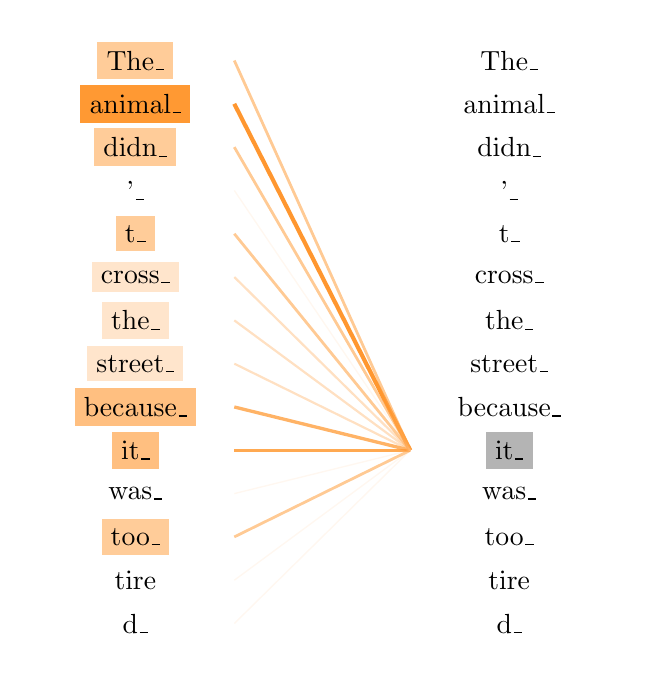
\begin{tikzpicture}[
    word/.style={minimum width=2.5cm, minimum height=0.6cm, text centered},
    highlight/.style={fill=orange!30},
    strongesthighlight/.style={fill=orange!80},
    stronghighlight/.style={fill=orange!50},
    mediumhighlight/.style={fill=orange!40},
    weakerhighlight/.style={fill=orange!20},
    attentiontarget/.style={fill=attentiontarget},
    node distance=0mm
]

% Left column
\matrix (left) [matrix of nodes, nodes={word}, row sep=-0.5mm, column sep=0mm] {
    The\_ \\
    animal\_ \\
    didn\_ \\
    '\_ \\
    t\_ \\
    cross\_ \\
    the\_ \\
    street\_ \\
    because\_ \\
    it\_ \\
    was\_ \\
    too\_ \\
    tire \\
    d\_ \\
};

% Right column
\matrix (right) [matrix of nodes, nodes={word}, right=2cm of left, row sep=-0.5mm, column sep=0mm] {
    The\_ \\
    animal\_ \\
    didn\_ \\
    '\_ \\
    t\_ \\
    cross\_ \\
    the\_ \\
    street\_ \\
    because\_ \\
    it\_ \\
    was\_ \\
    too\_ \\
    tire \\
    d\_ \\
};

% Apply highlighting to specific cells with better gradation
\node[strongesthighlight] at (left-2-1) {animal\_};
\node[stronghighlight] at (left-10-1) {it\_};
\node[stronghighlight] at (left-9-1) {because\_};
\node[mediumhighlight] at (left-1-1) {The\_};
\node[mediumhighlight] at (left-3-1) {didn\_};
\node[mediumhighlight] at (left-5-1) {t\_};
\node[mediumhighlight] at (left-12-1) {too\_};
\node[weakerhighlight] at (left-6-1) {cross\_};
\node[weakerhighlight] at (left-7-1) {the\_};
\node[weakerhighlight] at (left-8-1) {street\_};

\node[attentiontarget] at (right-10-1) {it\_};

% Draw connection lines with better opacity gradation
% Most important connection - animal to it
\draw[orange!90, opacity=0.9, line width=1.5pt] (left-2-1.east) to (right-10-1.west);

% Strong connections
\draw[orange!85, opacity=0.8, line width=1.2pt] (left-10-1.east) to (right-10-1.west);
\draw[orange!80, opacity=0.75, line width=1.2pt] (left-9-1.east) to (right-10-1.west);

% Medium connections
\draw[orange!70, opacity=0.6, line width=1pt] (left-1-1.east) to (right-10-1.west);
\draw[orange!70, opacity=0.6, line width=1pt] (left-3-1.east) to (right-10-1.west);
\draw[orange!70, opacity=0.6, line width=1pt] (left-5-1.east) to (right-10-1.west);
\draw[orange!70, opacity=0.6, line width=1pt] (left-12-1.east) to (right-10-1.west);

% Weaker connections
\draw[orange!60, opacity=0.4, line width=0.8pt] (left-6-1.east) to (right-10-1.west);
\draw[orange!60, opacity=0.4, line width=0.8pt] (left-7-1.east) to (right-10-1.west);
\draw[orange!60, opacity=0.4, line width=0.8pt] (left-8-1.east) to (right-10-1.west);

% Weakest connections
\foreach \i in {4,11,13,14} {
    \draw[orange!40, opacity=0.15, line width=0.5pt] (left-\i-1.east) to (right-10-1.west);
}

\end{tikzpicture}
\end{center}

You sometimes do want this, but mostly you don't.
The reason is that most of the time you're trying to predict the next token, based on the previous tokens.
So you want the representation for ``it\_'' to depend on just the previous tokens (and itself).
This is ``causal self-attention''.
In causal self-attention, token $i$ doesn't attend to any tokens in future, i.e.\
\begin{align}
  A^\text{causal}_{i<j} &= 0.
\end{align}
Diagramatically,
\begin{center}
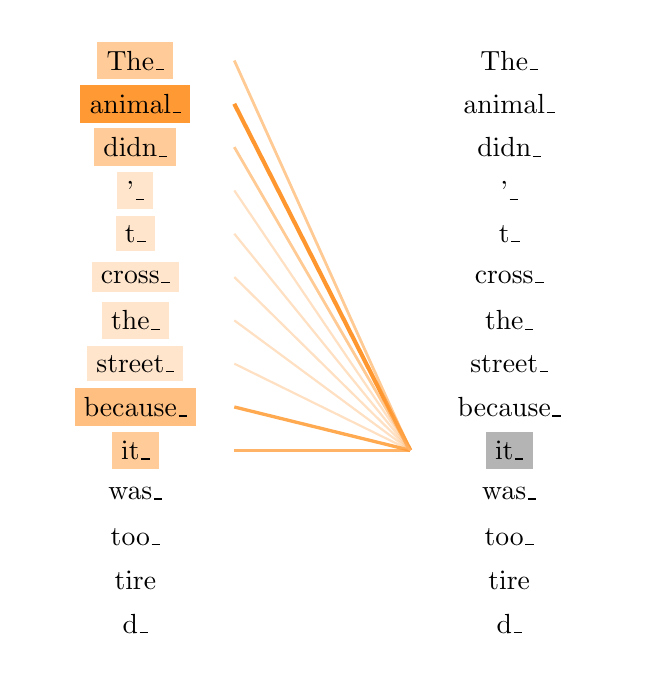
\begin{tikzpicture}[
    word/.style={minimum width=2.5cm, minimum height=0.6cm, text centered},
    highlight/.style={fill=orange!30},
    strongesthighlight/.style={fill=orange!80},
    stronghighlight/.style={fill=orange!50},
    mediumhighlight/.style={fill=orange!40},
    weakerhighlight/.style={fill=orange!20},
    attentiontarget/.style={fill=attentiontarget},
    node distance=0mm
]

% Left column (source tokens)
\matrix (left) [matrix of nodes, nodes={word}, row sep=-0.5mm, column sep=0mm] {
    The\_ \\
    animal\_ \\
    didn\_ \\
    '\_ \\
    t\_ \\
    cross\_ \\
    the\_ \\
    street\_ \\
    because\_ \\
    it\_ \\
    was\_ \\
    too\_ \\
    tire \\
    d\_ \\
};

% Right column (target token - "it_")
\matrix (right) [matrix of nodes, nodes={word}, right=2cm of left, row sep=-0.5mm, column sep=0mm] {
    The\_ \\
    animal\_ \\
    didn\_ \\
    '\_ \\
    t\_ \\
    cross\_ \\
    the\_ \\
    street\_ \\
    because\_ \\
    it\_ \\
    was\_ \\
    too\_ \\
    tire \\
    d\_ \\
};

% Highlight the "it_" token in the right column
\node[attentiontarget] at (right-10-1) {it\_};

% Apply highlighting to tokens up to and including "it_" with different intensities
\node[strongesthighlight] at (left-2-1) {animal\_};
\node[stronghighlight] at (left-9-1) {because\_};
\node[mediumhighlight] at (left-1-1) {The\_};
\node[mediumhighlight] at (left-3-1) {didn\_};
\node[mediumhighlight] at (left-10-1) {it\_};
\node[weakerhighlight] at (left-5-1) {t\_};
\node[weakerhighlight] at (left-6-1) {cross\_};
\node[weakerhighlight] at (left-7-1) {the\_};
\node[weakerhighlight] at (left-8-1) {street\_};
\node[weakerhighlight] at (left-4-1) {'\_};

% Draw connection lines - causal self-attention (only connections to itself and previous tokens)
% Most important connection - animal to it
\draw[orange!90, opacity=0.9, line width=1.5pt] (left-2-1.east) to (right-10-1.west);

% Strong connection - because to it (just before it)
\draw[orange!85, opacity=0.8, line width=1.2pt] (left-9-1.east) to (right-10-1.west);

% Medium strong connection - it to itself
\draw[orange!80, opacity=0.75, line width=1.2pt] (left-10-1.east) to (right-10-1.west);

% Medium connections
\draw[orange!70, opacity=0.6, line width=1pt] (left-1-1.east) to (right-10-1.west);
\draw[orange!70, opacity=0.6, line width=1pt] (left-3-1.east) to (right-10-1.west);

% Weaker connections
\draw[orange!60, opacity=0.4, line width=0.8pt] (left-5-1.east) to (right-10-1.west);
\draw[orange!60, opacity=0.4, line width=0.8pt] (left-6-1.east) to (right-10-1.west);
\draw[orange!60, opacity=0.4, line width=0.8pt] (left-7-1.east) to (right-10-1.west);
\draw[orange!60, opacity=0.4, line width=0.8pt] (left-8-1.east) to (right-10-1.west);
\draw[orange!60, opacity=0.4, line width=0.8pt] (left-4-1.east) to (right-10-1.west);
\end{tikzpicture}
\end{center}
Causal self-attention is implemented using a \textit{mask} in the attention matrix, which masks out future tokens,
\begin{align}
  A^\text{causal}_{ij}(\mathbf{Q}, \mathbf{K}) &=  \frac{\mathbb{I}(j \leq i) \exp(\mathbf{Q}_{i, :} \cdot \mathbf{K}_{j, :})}{\sum_k \mathbb{I}(k \leq i) \exp(\mathbf{Q}_{i, :} \cdot \mathbf{K}_{k, :})}
  \intertext{where $\mathbb{I}$ is the indicator function, which is $1$ when the condition holds, and $0$ otherwise, i.e.}
  \mathbb{I}(j \leq i) &= \begin{cases}
    1 &\text{if } j \leq i\\
    0 &\text{otherwise}.
  \end{cases}
\end{align}

\section{Training vs generation}

Generation is when you actually generate tokens:
\begin{itemize}
  \item You generate the next token, based on the previous tokens.
  \item You feed this new token into the model as well, and generate the next token.
  \item etc.
\end{itemize}
Thus if we started with 10 tokens and had to generate tokens 10 to 20, the code would look something like:
\begin{verbatim}
#High-level structure of code for generation
for token_index in range(10, 20):
    for layer_index in range(layers):
        ...
\end{verbatim}
i.e.\ the ``outer for loop'' ranges over tokens.
However, that means there's \verb|number_of_tokens| $\times$ \verb|number_of_layers| operations, which can be very slow.
When we're generating, there's no way to get away from this slowness.

But for training, you can avoid the slowness!
In particular, when you're training, you don't need to generate the next token: your training data tells you what the next token is!
As such, because of the causal masking in the self-attention, the representation of any token at any position in the transformer only depends on previous tokens.
That means, you can parallelise across token indices using efficient tensor operations (like causal self-attention and matrix multiplications), without an explicit ``for loop'' across token indices.
Instead, the outer for loop is just over layers:
\begin{verbatim}
#High-level structure of code for training
for layer_index in range(layers):
    ...
\end{verbatim}
Which is far more efficient.
To get some intuition on why this is possible, take the string below ``The cat sat on the mat and purred''.
You can simultaneously consider predicting any given token from the previous tokens.
An example is given below:

\begin{center}
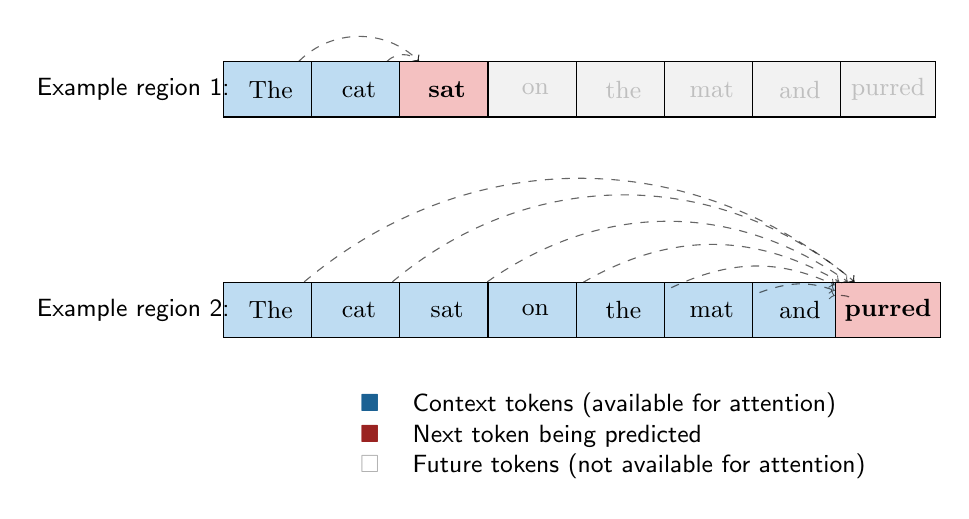
\begin{tikzpicture}[
    scale=0.8,
    token/.style={rectangle, minimum width=1.2cm, minimum height=0.7cm, draw, fill=white, align=center, font=\small},
    context-token/.style={rectangle, minimum width=1.2cm, minimum height=0.7cm, draw, fill=blue!30, align=center, font=\small},
    next-token/.style={rectangle, minimum width=1.2cm, minimum height=0.7cm, draw, fill=red!30, align=center, font=\small\bfseries},
    future-token/.style={rectangle, minimum width=1.2cm, minimum height=0.7cm, draw, fill=gray!10, align=center, text=gray!50, font=\small},
    annotation/.style={align=left, font=\small\sffamily},
    attention-arrow/.style={->, thin, dashed, black, opacity=0.6}
]

% First string - Region 1
\node[context-token] (t1a) at (0,2) {The};
\node[context-token] (t2a) at (1.4,2) {cat};
\node[next-token] (t3a) at (2.8,2) {sat};
\node[future-token] (t4a) at (4.2,2) {on};
\node[future-token] (t5a) at (5.6,2) {the};
\node[future-token] (t6a) at (7.0,2) {mat};
\node[future-token] (t7a) at (8.4,2) {and};
\node[future-token] (t8a) at (9.8,2) {purred};

% Second string - Region 2
\node[context-token] (t1b) at (0,-1.5) {The};
\node[context-token] (t2b) at (1.4,-1.5) {cat};
\node[context-token] (t3b) at (2.8,-1.5) {sat};
\node[context-token] (t4b) at (4.2,-1.5) {on};
\node[context-token] (t5b) at (5.6,-1.5) {the};
\node[context-token] (t6b) at (7.0,-1.5) {mat};
\node[context-token] (t7b) at (8.4,-1.5) {and};
\node[next-token] (t8b) at (9.8,-1.5) {purred};

% Draw causal attention arrows
% First string - Region 1
\draw[attention-arrow] (t1a) to[out=45, in=135] (t3a);
\draw[attention-arrow] (t2a) to[out=45, in=135] (t3a);

% Second string - Region 2
\draw[attention-arrow] (t1b) to[out=40, in=140] (t8b);
\draw[attention-arrow] (t2b) to[out=40, in=140] (t8b);
\draw[attention-arrow] (t3b) to[out=35, in=145] (t8b);
\draw[attention-arrow] (t4b) to[out=30, in=150] (t8b);
\draw[attention-arrow] (t5b) to[out=25, in=155] (t8b);
\draw[attention-arrow] (t6b) to[out=20, in=160] (t8b);
\draw[attention-arrow] (t7b) to[out=15, in=165] (t8b);

% Annotations
\node[annotation, anchor=east] (note1) at (-0.5,2) {Example region 1:};
\node[annotation, anchor=east] (note2) at (-0.5,-1.5) {Example region 2:};

% Legend
\node[annotation, anchor=west] at (1,-3.5) {
\begin{tabular}{ll}
\textcolor{blue!70!black}{$\blacksquare$} & Context tokens (available for attention) \\
\textcolor{red!70!black}{$\blacksquare$} & Next token being predicted \\
\textcolor{gray!60}{$\square$} & Future tokens (not available for attention) \\
\end{tabular}
};

\end{tikzpicture}
\end{center}


\end{document}

